\documentclass[12pt]{article}
\usepackage{graphicx}
\usepackage{listings}
\usepackage{times}
\usepackage{amsmath,amsthm, amssymb, latexsym}
\usepackage[abbr]{harvard}
\usepackage{hyperref}

%\hypersetup{urlcolor=cyan}

\newcommand{\link}[2]{\href{#1}{\textcolor{blue}{\underline{#2}}}}
\newcommand{\code}{http://www.cc.gatech.edu/~simpkins/teaching/gatech/cs2316/code}


\usepackage{color}
\definecolor{dkgreen}{rgb}{0,0.6,0}
\definecolor{gray}{rgb}{0.5,0.5,0.5}
\definecolor{mauve}{rgb}{0.58,0,0.82}

\usepackage{listings}
% Default settings for code listings
\lstset{frame=tb,
  aboveskip=3mm,
  belowskip=3mm,
  showstringspaces=false,
  columns=flexible,
  basicstyle={\scriptsize\ttfamily},
  numbers=none,
  numberstyle=\tiny\color{gray},
  keywordstyle=\color{blue},
  commentstyle=\color{dkgreen},
  stringstyle=\color{mauve},
  frame=single,
  breaklines=true,
  breakatwhitespace=true
}


\textwidth = 6.5 in
\textheight = 9.5 in
\oddsidemargin = 0.0 in
\evensidemargin = 0.0 in
\topmargin = -0.25 in
\headheight = 0.0 in
\headsep = 0.0 in
\parskip = 0.0 in
\parindent = 0.0in
\itemsep = 0in

\title{Hangman}
\author{}
\date{}

\begin{document}

\maketitle
\vspace{-1in}
\section{Introduction}

In this assignment you will practice
\begin{itemize}
\itemsep0em
\item writing Python programs and modules,
\item writing programs and modules that use other modules,
\item using control structures,
\item validating user input and dealing with invalid input,
\item using data structures and string processing, and
\item writing interactive console programs.
\end{itemize}

\section{Problem Description}

You like word-guessing games.

\section{Solution Description}

Write a Python program that implements the classic Hangman game.  Game play proceeds as follows:

\begin{enumerate}
\item The hangman program asks the user what kind of word they want to guess, e.g., "hard", "easy".
\item The hangman program chooses a word at random from the approprite list and displays the number of letters in the word in the form of a number of underlines (spaces to be filled in).
\item As long as the hangman is not complete or the user has not guessed all the letters in the word:
\begin{enumerate}
\item The program asks the user to guess a letter.
\item The user enters a letter and presses return.
\item If the user enters more than one letter or a non-letter, tell the user to enter only one letter and try again.
\item If the user's guess is in the word, the letter is placed in the appropriate blanks (can be more than one occurrence in the word); otherwise a new body part is drawn on the hangman.
\item If, after the user's guess, the word is completely revealed, the user wins and the game is over.  Report this to the user and exit.
\item If, after the user's guess, the hangman is complete (head, body, arms, legs, etc.), the user loses and the game is over.  Report this to the user and exit.
\end{enumerate}
\end{enumerate}

Your program should use two provided modules, {\tt drawing} and {\tt words}, both located in the {\tt hanglib} package.  Instructions for downloading these files follow.

\begin{enumerate}
\itemsep0em
\item Create a {\tt hw1} subdirectory of your CS2316 coursework directory for your HW1 solution.
\item Create a {\tt hanglib} subdirectory of your {\tt hw1} directory.
\item Download \link{\code/hanglib/drawing.py}{drawing.py} and \link{\code/hanglib/words.py}{words.py} into your {\tt hanglib} directory.
\end{enumerate}

You will write three Python files (in your {\tt hw1} directory):

\begin{enumerate}
\itemsep0em
\item {\tt extraparts.py} -- a module that draws additional body parts on the hangman drawn by \link{\code/hanglib/drawing.py}{drawing.py}.  These can be facial features, hands, feet, or any creative non-lewd idea of your own.
\item {\tt extrawords.py} -- a module containing additional word lists, named by type of word.  Again, use your creativity.
\item {\tt hangman.py} -- a program that implements the hangman game using the provided modules and the two you create yourself.
\end{enumerate}

A finished hangman program will look something like this:

\begin{tabular}{cc}
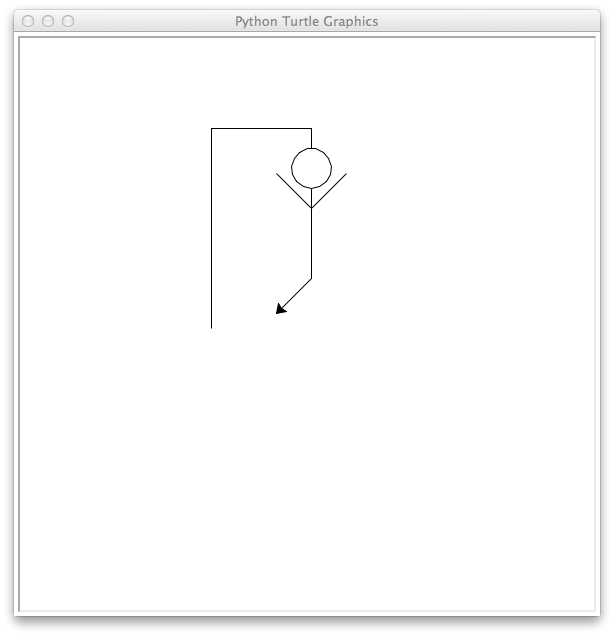
\includegraphics[width=3in]{hangman-fig.png} &
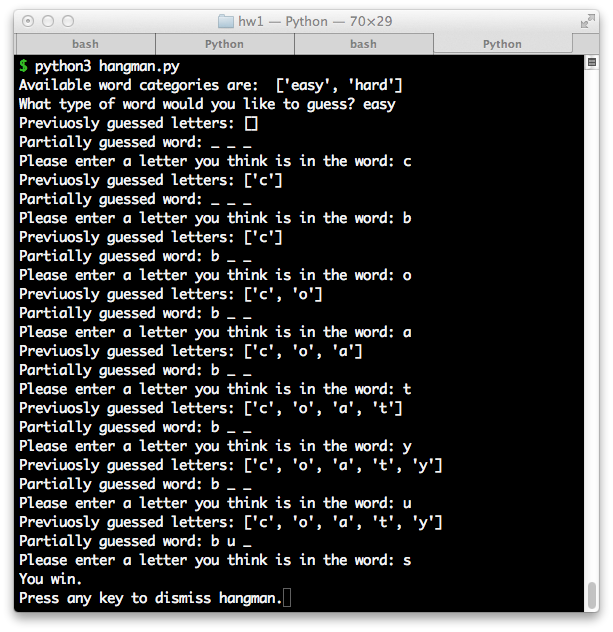
\includegraphics[width=3in]{hangman-console.png}
\end{tabular}

\section{Tips}

\begin{itemize}
\itemsep0em
\item Remember that functions are first-class objects.  So you could have a list of functions, e.g., {\tt parts = [draw.head, draw.body]} and call {\tt draw.head} with {\tt parts[0]()}.
\item The {\tt range()} function returns an interator over a range of integers.  For example, if you have a list of elements, {\tt xs}, {\tt range(len(xs))} returns an iterator over the indexes of {\tt xs}. See \link{https://docs.python.org/3/library/functions.html}{built-in functions docs}.
\item Python's standard {\tt random} module's {\tt choice(seq)} function returns a randomly chosen element from {\tt seq}.  See \link{https://docs.python.org/3/library/random.html}{random module docs}.
\item At the end of the game, ask the user to press a key to dismiss the hangman with the {\tt input()} function.  Otherwise the turtle window with the hangman will disappear immediately.
\end{itemize}

\section{Turn-in Procedure}

Submit your {\tt hangman.py}, {\tt extraparts.py} and {\tt extrawords.py} files on T-Square as three separate attachments.  When you're ready, double-check that you have submitted and not just saved a draft.

\section{Verify the Success of Your Submission to T-Square}

Practice safe submission! Verify that your HW files were truly submitted correctly, the upload was successful, and that your program runs with no syntax or runtime errors. It is solely your responsibility to turn in your homework and practice this safe submission safeguard.

\begin{enumerate}
\itemsep0em
\item After uploading the files to T-Square you should receive an email from T-Square listing the names of the files that were uploaded and received. If you do not get the confirmation email almost immediately, something is wrong with your HW submission and/or your email. Even receiving the email does not guarantee that you turned in exactly what you intended.
\item After submitting the files to T-Square, return to the Assignment menu option and this homework. It should show the submitted files.
\item Download copies of your submitted files from the T-Square Assignment page placing them in a new folder.
\item Re-run and test the files you downloaded from T-Square to make sure it's what you expect.
\item This procedure helps guard against a few things.
\begin{enumerate}
\itemsep0em
\item It helps insure that you turn in the correct files.
\item It helps you realize if you omit a file or files.\footnote{Missing files will not be given any credit, and non-compiling homework solutions will receive few to zero points. Also recall that late homework will not be accepted regardless of excuse. Treat the due date with respect.  Do not wait until the last minute!}
(If you do discover that you omitted a file, submit all of your files again, not just the missing one.)
\item Helps find syntax errors or runtime errors that you may have added after you last tested your code.
\end{enumerate}
\end{enumerate}

\end{document}
